\documentclass{article}
\usepackage[british]{babel}
\usepackage[utf8]{inputenc}
\usepackage{fancyhdr}
\usepackage{lastpage}
\usepackage{amssymb}
\usepackage{amsmath}
\usepackage{amsfonts}
\usepackage{amsthm}
\usepackage{wasysym}
\usepackage{ulem}
\usepackage[shortlabels]{enumitem}
\usepackage{multicol}
\usepackage{biblatex}
\usepackage{csquotes}
\usepackage{graphicx}
\usepackage{algorithm}
\usepackage{algorithmic}
\usepackage[a4paper, total={5.25in, 8in}]{geometry}
\addbibresource{refs.bib}

\makeatletter
\renewenvironment{proof}[1][\proofname]{\par
\pushQED{\qed}%
\normalfont \topsep6\p@\@plus6\p@\relax
\trivlist
\item\relax
{\itshape\bfseries
#1\@addpunct{.}}\hspace\labelsep\ignorespaces
}{%
\popQED\endtrivlist\@endpefalse
}
\makeatother

\DeclareFieldFormat*{titlecase}{
    \ifdef{\currentfield}
      {\ifcurrentfield{title}
         {\usefield{\uline}{\currentfield}}%
         {#1}}
      {#1}}
\DeclareFieldFormat*{title}{#1}

% =============================================================================

\pagestyle{fancy}
\fancyhf{}
\rhead{Page \thepage \textrm{ of }\pageref{LastPage}}
\lhead{2009169 - CS331 Coursework}


\title{CS331 Neural Computing Coursework}
\author{Short Answer Questions}
\date{2009169}

% =============================================================================

\begin{document}

\maketitle
\thispagestyle{fancy}

\section*{Question 1}

\subsection*{A}

The derived logic gate \textit{imply}.

The truth table of the \textit{imply} gate is as follows:

\begin{center}
   \begin{tabular}{cc|c}
      $x_1$ & $x_2$ & $y$ \\
      \hline
      0 & 0 & 1\\
      0 & 1 & 1\\
      1 & 0 & 0\\
      1 & 1 & 1
   \end{tabular}
\end{center}

\textbf{\textit{Perceptron.}} Representing this graphically, we get positive coordinates at (0, 0), (0, 1), (1, 1), and negative coordinates at (1, 0).

The positive and negative regions can be split with a single straight line $x_1 - x_2 + 0.5 \leq 0$, thus we can use a single-layer perceptron with weights $(w_1, w_2) = (1, -1)$ and bias $b = 0.5$. \bigskip

\textbf{\textit{MP Neuron.}} Imply cannot be written with MP neuron:

\begin{itemize}
   \item When $x_1 = 0, x_2 = 0$, $y = 1$, thus threshold $\theta = 0$.
   \item When $x_1 = 0, x_2 = 1$, $y=1$, this agrees with $\theta = 0$.
   \item When $x_1 = 1, x_2 = 0$, $y = 0$, and since we must have $\theta = 0$, $x_1$ must inhibit. This agrees with the above.
   \item But when $x_1=1, x_2=1$, $y=1$, which means $x_1$ cannot inhibit.
\end{itemize}

Since this is a contradiction, \textit{imply} cannot be written with an MP neuron.

\subsection*{B}

Clustering is a type of unsupervised learning, whilst classification is supervised learning. 

That is -- in Clustering, we give no labels to the data, and the aim is to \textit{discover} labels for data, or ``clusters'' automatically. This allows us to learn underlying structures to data. \textit{K-means clustering} is an example of clustering, where we initialise a set of $k$ mean values, and the algorithm refines those means to find $k$ clusters.

In classification, we give labels to the data in classes, and the model refines itself based on correct lables to separate our given classes into their own categories. \textit{Logistic regression} is a type of classification with linear boundaries, using linear regression as its basis.

See figure [REF].

\textbf{Insert a picture of both here and remove this message.}

\subsection*{C}

Action potentials are transmitted between synapses using chemical signals. These chemicals are called neurotransmitters.

When an action potential is sent down the axon of the presynaptic neuron $p_n$, it causes the vesicles in its axon terminal to release the neurotransmitters through the membrane into the synaptic cleft. 

The neurotransmitters interact with and bind to receptors on the cell membrane of the postsynaptic neuron $p_{n+1}$, which may cause an action to occur, increasing the chance that $p_{n+1}$ may fire an action potential, or inhibiting it entirely.

\section*{Question 2}

\subsection*{A}

The network diagram can be found in figure \ref{fig:2l}.

\begin{figure}[t]
   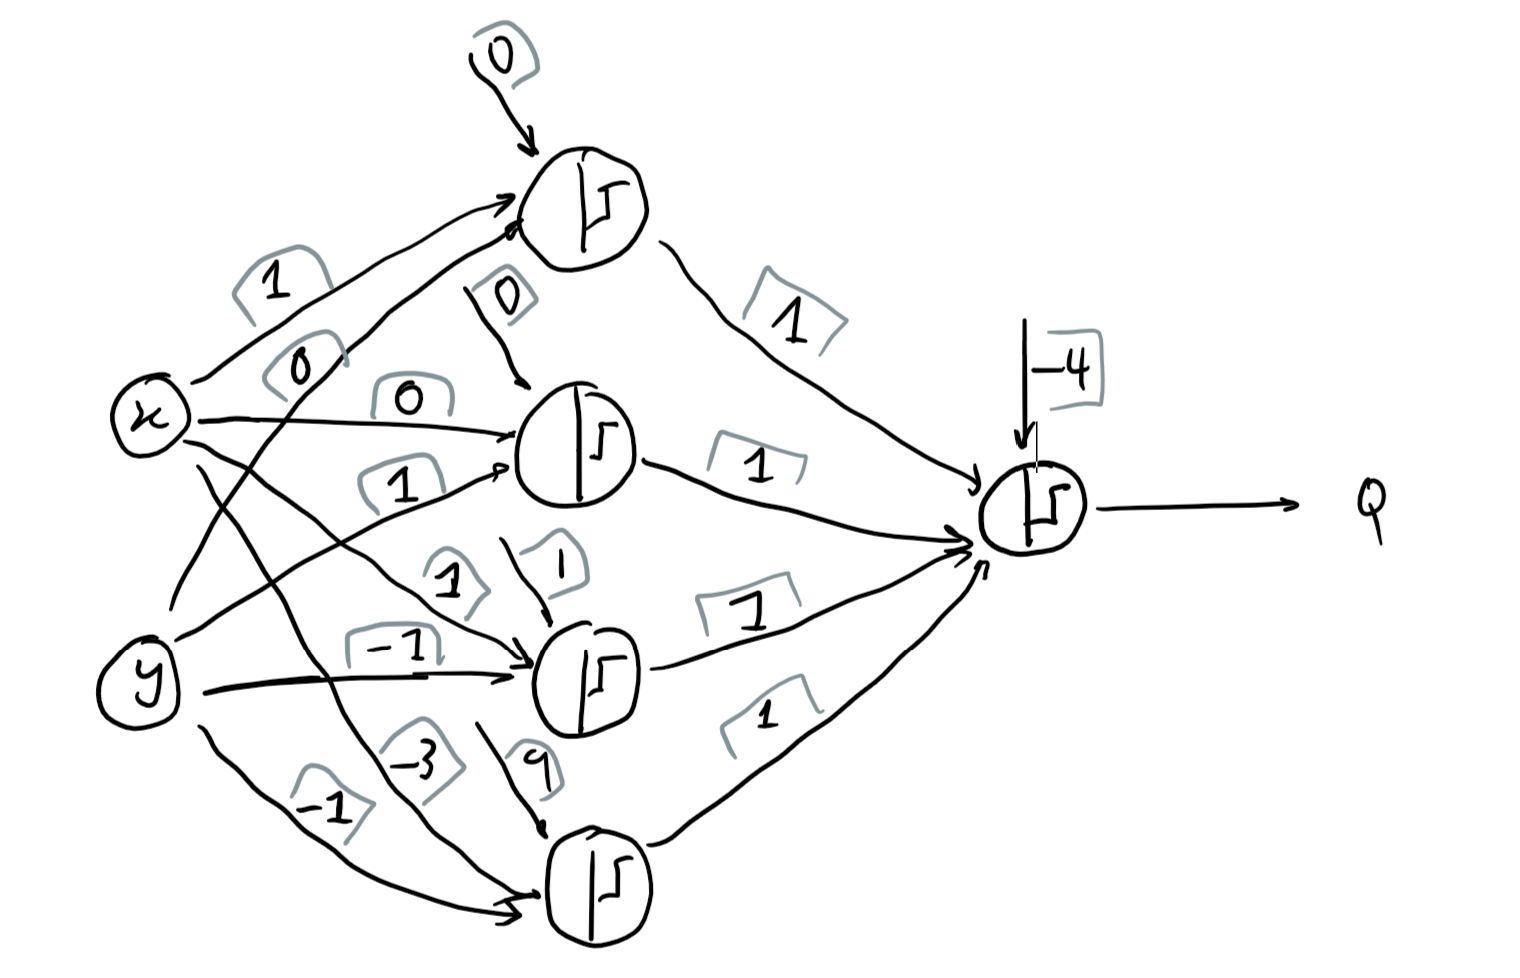
\includegraphics[width=0.6\textwidth]{2layerperc.png}
   \centering
   \caption[]{Two later perceptron for Q 2.A}
   \label{fig:2l}
\end{figure}

The shaded area is a quadrilateral made of four half-planes, ANDed together. Thus, we have:

\begin{itemize}
   \item $x \geq 0 \implies 1x + 0y + 0 \geq 0$
   \item $y \geq 0 \implies 0x + 1y + 0 \geq 0$
   \item $y \leq x + 1 \implies 1x - 1y + 1 \geq 0$
   \item $y \leq -3x + 9 \implies -3x -1y + 9 \geq 0$
\end{itemize}

The co-efficients of which give the weights and biases.

\subsection*{B}

The \textit{sigmoid} function has a few limitations, including being computationally expensive (due to the $e^{-x}$) and not being zero-centred. Most importantly though, sigmoid suffers greatly from the \textit{vanishing gradient} problem, where since the gradient is relatively flat far away from zero, a network cannot learn quickly. 

The easiest way to avoid this vanishing gradient at large values is to use ReLU. Simultaneously this also solves computational complexity, as ReLU is very quick.

The \textit{ReLU} function also has limitations however, being not zero-centered, not differentiable at zero, but most importantly having zero gradient any time $x < 0$. This is referred to as a dead ReLU.

To solve this we can use \textit{Leaky ReLU} instead of ReLU. Whilst regular ReLU has $h(x) = \max(0, x)$, Leaky ReLU has $h(x) = \max(\alpha x, x)$ for some small value $\alpha$, thus allowing negative values to ``leak'' some of their gradient out, meaning that whilst gradients for $x < 0$ are not large, they are not zero.

\subsection*{C}

\section*{Question 3}

\subsection*{A}

\subsection*{B}

\subsection*{C}

\end{document}